\documentclass[a4paper]{article}
\usepackage{a4wide}
\usepackage{amsmath}
\usepackage{amssymb}
\usepackage{dsfont}
\pagestyle{plain}
\usepackage{tikz}
\usetikzlibrary{matrix}
\usepackage{eurosym}
\usepackage{amsthm}
\usepackage{mathrsfs}
\usepackage{dlfltxbcodetips}
\usepackage{cancel}
\usepackage{bbm}
\usepackage{graphicx}
%    \usepackage{tkz-graph}  
%    \usetikzlibrary{shapes.geometric}%   
% 	 \usetikzlibrary{bayesnet}
	
%\documentclass[12pt]{article}

\usepackage[utf8]{inputenc} % UTF8-Kodierung für Umlaute usw
% \usepackage[ngerman]{babel} % Sprache: Deutsch
\usepackage{graphicx}

\usepackage[margin=1in]{geometry}
\usepackage{array}
\usepackage{amsthm,amssymb}
%\usepackage[fleqn]{amsmath}

\usepackage{multicol}

\newcommand*{\carry}[1][1]{\overset{#1}}
\newcolumntype{B}[1]{r*{#1}{@{\,}r}}

\newcommand{\N}{\mathbb{N}}
\newcommand{\Z}{\mathbb{Z}}

\newcommand{\extitle}[1]{{\vspace{5mm}\Large\b{#1}}\vspace{2mm}\\}
\newcommand{\exsubtitle}[1]{{\large\b{#1}}\vspace{2mm}\\}

\renewcommand*{\i}[1]{{\textit{#1}}}
\renewcommand*{\b}[1]{{\textbf{#1}}}
\renewcommand*{\tt}[1]{{\texttt{#1}}}

\setlength{\parindent}{0cm}
%\setlength{\mathindent}{0cm}
 % import config
\DeclareMathOperator*{\argmax}{arg\,max}
\DeclareMathOperator*{\argmin}{arg\,min}  
\newcommand{\norm}[1]{\left\lVert#1\right\rVert}
\newcommand{\vivid}{\stackrel{\text{vivid}}{=}}
\newcommand{\icol}[1]{% inline column vector
  \left(\begin{smallmatrix}#1\end{smallmatrix}\right)%
}

\newcommand\indep{\protect\mathpalette{\protect\indeP}{\perp}}
\def\indeP#1#2{\mathrel{\rlap{$#1#2$}\mkern2mu{#1#2}}}

\newcommand{\mlq}{F(\q)}
\newcommand{\si}{s}
\newcommand{\sj}{{s'}}
\newcommand{\p}{p}
\newcommand{\q}{r}
\newcommand{\z}{w}
%\newcommand{\x}{\mathcal{D}}
%\newcommand{\mlq}{-L(\q)}
%\newcommand{\si}{i}
%\newcommand{\sj}{j}
%\newcommand{\p}{p}
%\newcommand{\q}{q}
%\newcommand{\z}{Z}
%\newcommand{\x}{X}

\newcommand{\pxgz}{\p(\x|\z)}
\newcommand{\pzgx}{\p(\z|\x)}
\newcommand{\pxz}{\p(\x,\z)}
\newcommand{\px}{\p(\x)}

\newcommand{\qz}{\q(\z)}
\newcommand{\qi}{\q_\si}
\newcommand{\qj}{\q_\sj}
\newcommand{\qk}{\q_k}
\newcommand{\pz}{\p(\z)}
\newcommand{\pzi}{\p(\z_\si)}
\newcommand{\pzj}{\p(\z_\sj)}
\newcommand{\pzk}{\p(\z_k)}

\newcommand{\sigm}{\text{sigm}}

\newcommand{\zi}{\z_\si}
\newcommand{\zj}{\z_\sj}
\newcommand{\zk}{\z_k}
\newcommand{\dz}{\mathrm{d}\z}
\newcommand{\dzi}{\mathrm{d}\z_\si}
\newcommand{\dzj}{\mathrm{d}\z_\sj}
\newcommand{\dzk}{\mathrm{d}\z_k} 

\newcommand{\E}{\mathbb{E}}





%\newcommand{\propq}{ \underset{ \text{wrt.}\put(1,1){\scriptsize *}q }{\propto} }

\newcommand{\eqs}[1]{ \stackrel{#1}{=}  }
\newcommand{\eqq}{  \overset{\text{!}}{=} }
\newcommand{\propqz}{ \underset{ \overset{\text{wrt.}}{\qz} }{\propto} }
\newcommand{\propz}{ \underset{ \overset{\text{wrt.}}{\z} }{\propto} }
\newcommand{\propzj}{ \underset{ \overset{\text{wrt.}}{\zj} }{\propto} }
%\newcommand{\constw}{ \underset{ \text{ wrt. \w} }{\text{ const}} }
%\newcommand{\consty}{ \underset{ \text{ wrt. \y} }{\text{ const}} }
\newcommand{\const}[1]{{\underset{ \text{ wrt. #1} }{\text{ const}} }}

\newcommand{\tr}[1]{{#1^\top}}
\newcommand{\inv}[1]{{#1^{-1}}}
\newcommand{\trk}[1]{{(#1)^\top}}
\newcommand{\invk}[1]{{(#1)^{-1}}}
\newcommand{\tin}[1]{{(#1^\top)^{-1}}}

\newcommand{\Yt}{{Y^\top}}
\newcommand{\Xt}{{X^\top}}
\newcommand{\xt}{{\x^\top}}
\newcommand{\yt}{{\y^\top}}
\newcommand{\Wt}{{\W^\top}}
\newcommand{\w}{w}
\newcommand{\lx}{{\lambda_{x}}}
\newcommand{\ly}{{\lambda_{y}}}
\newcommand{\rhi}{{r^{(i)}}}
\newcommand{\rhj}{{r^{(j)}}}
\newcommand{\xhi}{{x^{(i)}}}
\newcommand{\shi}{{s^{(i)}}}
\newcommand{\xhj}{{x^{(j)}}}
\newcommand{\shj}{{s^{(j)}}}
\newcommand{\Wi}{{W_{i}}}
\newcommand{\Wj}{{W_{j}}}
\newcommand{\Wit}{W_{i}^\top}
\newcommand{\Wjt}{W_{j}^\top}
\newcommand{\Wij}{W_{ij}}
\newcommand{\Wlk}{W_{lk}}
\newcommand{\ax}{{\alpha_{x}}}
\newcommand{\ay}{{\alpha_{y}}}
\newcommand{\axt}{\alpha_{x}^\top}
\newcommand{\ayt}{\alpha_{y}^\top}
\newcommand{\Cxx}{C_{xx}}
\newcommand{\Cxy}{C_{xy}}
\newcommand{\Cyx}{C_{yx}} 
\newcommand{\Cyy}{C_{yy}}
\newcommand{\1}{\mathds{1}}
\newcommand{\lag}{\mathcal{L}}


\begin{document}

% header configuration
\title{\b{Exercise Sheet 8}}
\author{Machine Learning 2, SS16}

\maketitle

% authors
Mario Tambos, 380599;\quad Viktor Jeney, 348969;\quad Sascha Huk, 321249;\quad Jan Tinapp, 0380549\\


\extitle{Exercise 2}
\begin{align*}
y_t=(w\ast x)_t=\sum_{s\in\mathbb{Z}}w_sx_{t-s}
\end{align*}
\textbf{(a)}\\
\begin{align*}
\frac{\partial E}{\partial x_k}
&=\sum_{t\in\mathbb{Z}}\frac{\partial E}{\partial y_t}\frac{\partial y_t}{\partial x_k}\\
&=\sum_{t\in\mathbb{Z}}\frac{\partial E}{\partial y_t}\frac{\partial}{\partial x_k}(w\ast x)_t\\
&=\sum_{t\in\mathbb{Z}}\frac{\partial E}{\partial y_t}\sum_{s\in\mathbb{Z}}w_s\frac{\partial}{\partial x_k}x_{t-s}\\
&=\sum_{t\in\mathbb{Z}}\frac{\partial E}{\partial y_t}\sum_{s\in\mathbb{Z}}w_s\mathbbm{1}_{\{t-s=k\}}\\
&=\sum_{t\in\mathbb{Z}}\frac{\partial E}{\partial y_t}w_{-k+t}\\
&=\left[\frac{\partial E}{\partial y}\star w\right]_{-k}
\end{align*}
\textbf{(b)}\\
\begin{align*}
\frac{\partial E}{\partial w_k}
&=\sum_{t\in\mathbb{Z}}\frac{\partial E}{\partial y_t}\frac{\partial y_t}{\partial w_k}\\
&=\sum_{t\in\mathbb{Z}}\frac{\partial E}{\partial y_t}\frac{\partial}{\partial w_k}(w\ast x)_t\\
&=\sum_{t\in\mathbb{Z}}\frac{\partial E}{\partial y_t}\sum_{s\in\mathbb{Z}} x_{t-s}\frac{\partial}{\partial w_k}w_s\\
&=\sum_{t\in\mathbb{Z}}\frac{\partial E}{\partial y_t}\sum_{s\in\mathbb{Z}}x_{t-s}\mathbbm{1}_{\{s=k\}}\\
&=\sum_{t\in\mathbb{Z}}\frac{\partial E}{\partial y_t}x_{-k+t}\\
&=\left[\frac{\partial E}{\partial y}\star x\right]_{-k}
\end{align*}
\extitle{Exercise 3}
\textbf{(a)}\\
Euler discretization gives us for every $j=1,..,d$:
\begin{align*}
x^t_j-x^{t-1}_j=0.1(\tanh(\sum_{i=1}^{d}x^{t-1}_i w_{ij}+b_j)-x^{t-1}_j)
\end{align*}
The transition function is then component wise defined as
\begin{align*}
\Theta(x)_j=0.1(\tanh(\sum_{i=1}^{d}x_i w_{ij}+b_j)-x_j)+x_j
\end{align*}

\textbf{(b)}\\
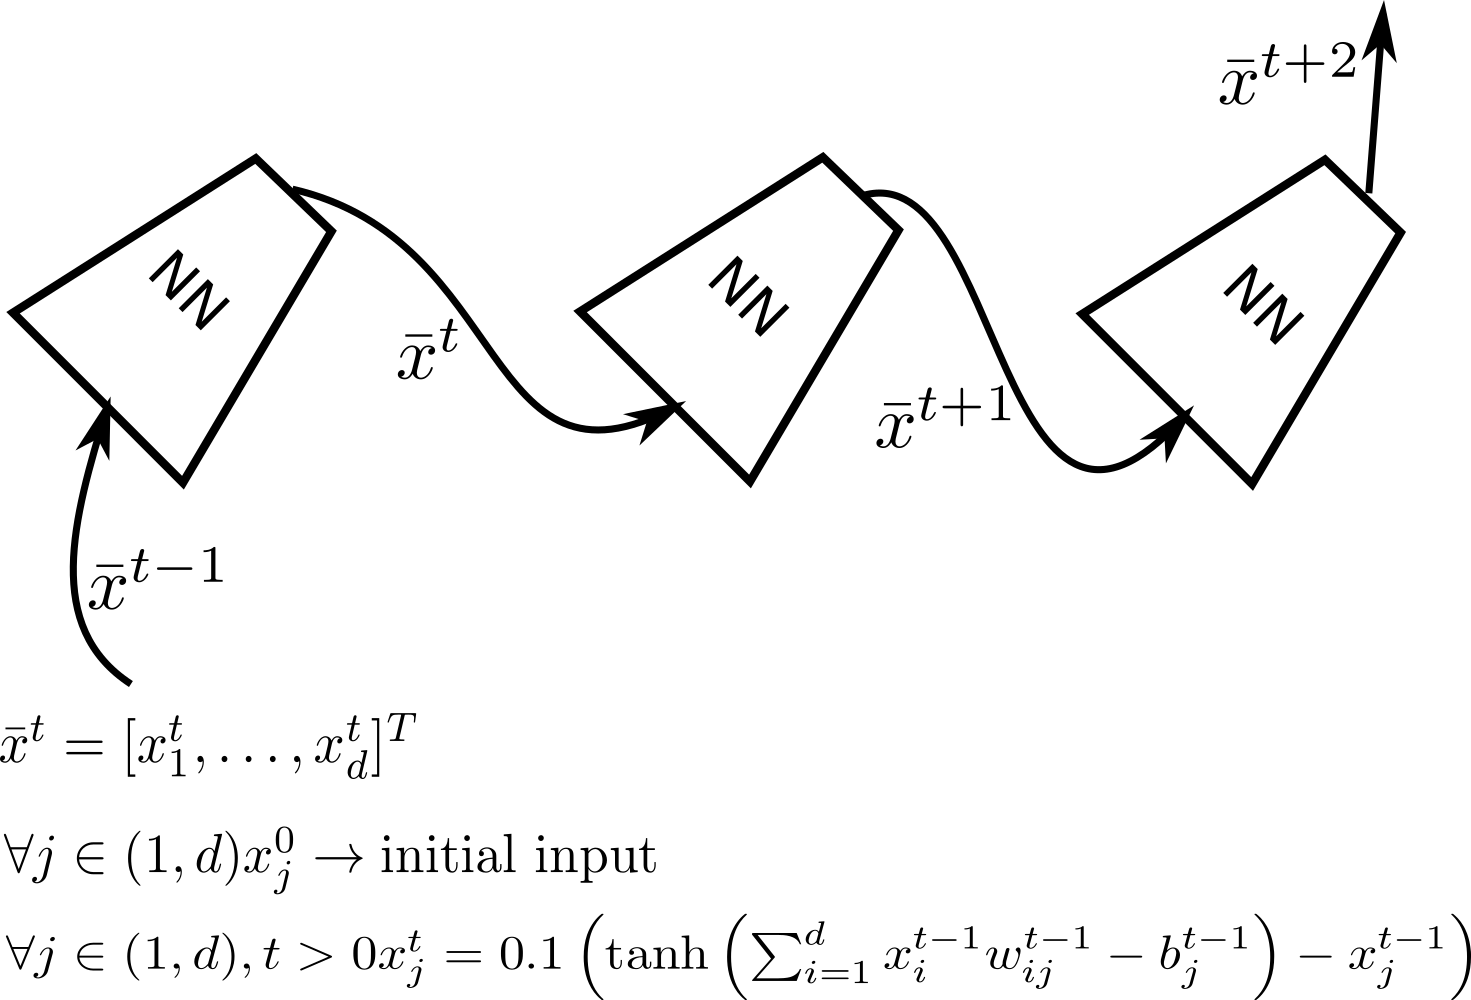
\includegraphics[width=0.7\textwidth]{nnet}\\
\includegraphics[width=0.7\textwidth]{nnet_time_step}
\\

\textbf{(c)}\\if you
\begin{align*}
\frac{\partial x^t_i}{\partial x^{t-1}_j}
&=0.1\frac{\partial}{\partial x^{t-1}_j}(\tanh(\sum_{k=1}^{d}x^{t-1}_k w_{ki}+b_i)-x^{t-1}_i)+\frac{\partial x^{t-1}_i}{\partial x^{t-1}_j}\\
&=0.1\frac{\partial}{\partial x^{t-1}_j}(\tanh(\sum_{k=1}^{d}x^{t-1}_k w_{ki}+b_i))+0.9\mathbbm{1}_{\{i=j\}}\\
&=0.1(1-\tanh(\sum_{k=1}^{d}x^{t-1}_k w_{ki}+b_i))\sum_{k=1}^{d}\frac{\partial}{\partial x^{t-1}_j}x^{t-1}_k w_{ki}+0.9\mathbbm{1}_{\{i=j\}}\\
&=0.1(1-\tanh(\sum_{k=1}^{d}x^{t-1}_k w_{ki}+b_i))\sum_{k=1}^{d}\mathbbm{1}_{\{k=j\}} w_{ki}+0.9\mathbbm{1}_{\{i=j\}}\\
&=0.1(1-\tanh(\sum_{k=1}^{d}x^{t-1}_k w_{ki}+b_i))w_{ji}+0.9\mathbbm{1}_{\{i=j\}}\\
\end{align*}
\textbf{(d)}\\
\begin{align*}
\frac{\partial x^t_i}{\partial b_j}
&=0.1\frac{\partial}{\partial b_j}\tanh(\sum_{k=1}^{d}x^{t-1}_k w_{ki}+b_i)\\
&=0.1(1-\tanh(\sum_{k=1}^{d}x^{t-1}_k w_{ki}+b_i))\frac{\partial b_i}{\partial b_j}\\
&=0.1(1-\tanh(\sum_{k=1}^{d}x^{t-1}_k w_{ki}+b_i))\mathbbm{1}_{\{i=j\}}\\
\end{align*}
\begin{align*}
\frac{\partial x^t_i}{\partial w_{jl}}
&=0.1\frac{\partial}{\partial w_{jl}}\tanh(\sum_{k=1}^{d}x^{t-1}_k w_{ki}+b_i)\\
&=0.1(1-\tanh(\sum_{k=1}^{d}x^{t-1}_k w_{ki}+b_i))\sum_{k=1}^{d}x^{t-1}_k\frac{\partial}{\partial w_{jl}}w_{ki}\\
&=0.1(1-\tanh(\sum_{k=1}^{d}x^{t-1}_k w_{ki}+b_i))\sum_{k=1}^{d}x^{t-1}_k\mathbbm{1}_{\{j=k\}}\mathbbm{1}_{\{l=i\}}\\
&=0.1(1-\tanh(\sum_{k=1}^{d}x^{t-1}_k w_{ki}+b_i))x^{t-1}_j\mathbbm{1}_{\{l=i\}}\\
\end{align*}
\end{document}






